\subsection{Ideal Curves}
One of the main concepts we learned this year in Multivariable Calculus, is finding the arc length of a curve. The formula for finding arc length of a curve is: \[\int_{a}^{b}\|\vec{c}^{\ \prime}(t)\|dt \text{ for } \vec{c}:[a, b] \rightarrow \R^{2}\]

We already know the paramaterization for Lissajous curves, so we can solve for $\|\vec{c}^{\ \prime}(t)\|$ through a short series of steps. We begin with our paramaterization: \[\vec{c}(t) = [A\sin(at+\delta),\ B\sin(bt)].\] From there, by differentiating both variables with respect to $t$, we see that \[\vec{c}^{\ \prime}(t) = [Aa\cos(at+\delta),\  Bb\cos(bt)].\] Then we can use Pythagoras' theorem to calculate the magnitude of c-prime. Doing so gives us: \[\|\vec{c}^{\ \prime}(t)\| = \sqrt{(Aa\cos(at+\delta))^2 + (Bb\cos(bt))^2}.\] Our integral now looks like this: \[\int_{t_0}^{t_f}\sqrt{(Aa\cos(at+\delta))^2 + (Bb\cos(bt))^2}\ dt\].

Before we can plug in our variables and evaluate, we need to solve for our bounds. Our lower bound is rather trivial, starting at $t=0$ unless special circumstances call for otherwise. Our upper bound is slightly more complicated. We can choose any time $t>0$, to find the arc length of the curve traced out until then, but eventually the curve will repeat itself. We can solve for what time the curve returns to it's initial position, which will allow us to find the arc length of the entire curve. To do so, we set the equation for $x$ and $y$ equal to their value at $t=0$: \[A\sin(at+\delta) = A\sin(\delta) \\ B\sin(bt) = 0.\] From the y equation, we know that $bt_f$ must be a multiple of $2\pi$. Let's look at an example: \[x=3\sin(4t),\ y=2\sin(3t).\]
\begin{center}
\begin{tikzpicture}[scale=0.8][h]
    \tkzInit[xmin=-4,xmax=4,xstep=1,ymin=-3,ymax=3,ystep=1]
    \tkzAxeX[step=1]
    \tkzAxeY[step=1,above]
    \tkzFctPar[color = purple, samples=200,domain=0:2*pi]{3*sin(4*t)}{2*sin(3*t)}
\end{tikzpicture}
\end{center}

In this example $t_f = 2\pi$, which means we can now integrate. For brevity, I will skip the steps for finding $\|\vec{c}^{\ \prime}(t)\|$ for this specific example and jump straight to the integral: \[\int_{0}^{2\pi}\sqrt{(12\cos(4t))^2 + (6\cos(3t))^2}\ dt \approx 56.2578.\]

\subsection{Real Curves}
The above work was for ideal Lissajous curves, but in the real world when we create the curves using harmonographs there's friction, which causes dampening in the curve. When we have dampening, we have to add a dampening factor to our parametric equations, when we do so, our new equations look like: \[x=A \sin (a t+\delta)e^{-dt}, \quad y=B \sin (b t)e^{-dt}\]

\begin{figure}[h]
\caption{Example of a Lissajous curve with and without dampening}
\begin{tikzpicture}[scale=0.8][h]
    \tkzInit[xmin=-2,xmax=2,xstep=1,ymin=-2,ymax=2,ystep=1]
    \tkzAxeX[step=1]
    \tkzAxeY[step=1,above]
    \tkzFctPar[color = red, samples=200,domain=0:2*pi]{sin(4*t)}{sin(3*t)}
    \tkzText[draw, text width=2.6cm, above, left, color = red, fill = red!20](-2,2){$x = \sin(4t) \\ y = \sin(3t)$}
\end{tikzpicture}
\begin{tikzpicture}[scale=0.8][h]
    \tkzInit[xmin=-2,xmax=2,xstep=1,ymin=-2,ymax=2,ystep=1]
    \tkzAxeX[step=1]
    \tkzAxeY[step=1,above]
    \tkzFctPar[color = blue, samples=1000,domain=0:100]{sin(4*t)*exp(-0.01*t)}{sin(3*t)*exp(-0.01*t)}
    \tkzText[draw, text width=3cm, above, left, color = blue, fill = blue!20](-1.5,2){$x = \sin(4t)e^{-0.01t} \\ y = \sin(3t)e^{-0.01t}$}
\end{tikzpicture}
\end{figure}
\newpage

Using this new paramaterization, we can recalculate the arc length. Following the same process as above, we can find that \[\|\vec{c}^{\ \prime}(t)\| = \sqrt{ (Aa\cos(at+\delta)e^{-dt} - dA\sin(at+\delta)e^{-dt})^2 +  (Bb\cos(bt)e^{-dt} - dB\sin(Bb)e^{-dt})^2}\] At this point before we solved for our bounds to integrate over, however because of the dampening there is no time where the curve returns to it's original position. In theory, the curve would continue forever without stopping, but calculus is all about evaluating at infinities, so we can still evaluate the integral as $t\rightarrow \infty$: \[\int_{0}^{\infty}\sqrt{ (Aa\cos(at+\delta)e^{-dt} - dA\sin(at+\delta)e^{-dt})^2 +  (Bb\cos(bt)e^{-dt} - dB\sin(bt)e^{-dt})^2}\ dt\] If we use the same example as above, but with a dampening factor of $d=-0.01$, our final integral to evaluate is: \[\int_{0}^{\infty}\sqrt{ (12\cos(4t)e^{-0.01t} - 0.03\sin(4t)e^{-0.01t})^2 +  (6\cos(3t)e^{-0.01t} - 0.02\sin(3t)e^{-0.01t})^2}\ dt\ \approx 895.37\]
